% !TeX root = ../Document.tex
\documentclass[../Document.tex]{subfiles}

\begin{document}
\section{Robot}
Upoznavši se sa tehnologijama, komponentama, detaljnim opisom uređaja i PID kontrolerom u dosadašnjem dijelu rada, imamo sve informacjie o potrebama za pravljenje samobalansirajućeg robota.

\subsection{Konstrukcija}
Konstrukciju robota čine 3 pločice pleksiglasa koje su namontirane na 4 navojne šike. Ispod same konstrukcije se nalaze 2 koračna motora sa točkovima. Pločice su raspoređene u spratove. Na prvome se nalazi matador ploča sa komponentama, na drugom Arduino Mega kontroler i na trećem spratu se ne nalazi ništa, već je njegova svrha dodati visinu samom robotu.

\subsubsection{Navojne šipke}
Navojne šipke su podrška čitavog robota. Četiri šipke dužine po 21cm daju robotu visinu koja ga dovodi u stanje disbalansa. Debljina svake šipke iznosi 4mm. U dužini šipke može postojati greška jer su rezane ručno.

\cFigure{Robot_Navojna-Sipka}{Navojna šipka}{0.5}

\subsubsection{Pleksiglas}
Pločice pleksiglasa na gornja dva sprata robota su debljine 3mm, dok je na prvom spratu debljina pločice 5mm kako bi mogla podnijeti težinu motora i točkova. Sve tri pločice imaju četiri rupe širine 4mm na svojim krajevima sa namjenom da se kroz njih provuku navojne šipke. Ono što ploče drži u mjestu i onemogućava im klizanje niz navojne šipke, (osim samog trenja) su matice postavljene ispod i iznad svake rupe u pločici (ukupno 24 matice). Pored toga, na pločici koja se nalazi na prvom spratu su također zabušene rupe veličine 4mm kroz koje su na pločicu pričvršćeni L-profili koji sa svoje druge strane imaju pričvršćene koračne motore. Srednji sprat na sebi ima zabušene četiri rupe veličine 3mm kroz koje su provučeni šarafi čiji je zadatak da drže Arduino MEGA pločicu pričvršćenom na mjestu.

\cFigure{Robot_Plexi}{Nacrt pleksiglas pločica sa rupama za navojne šipke}{0.8}

\subsubsection{Točkovi}
Točkovi koji se nalaze na koračnim motorima su plastični. Težina jednog točka je oko je oko 103g, a prečnik iznosi 144mm. Širina točka iznosi 45mm. Točkovi nisu savršeno proporcionalni, jer im svrha nije kontrolisati delikatnog robota, već se radi o pomoćnim točkovima za dječiji bicikl. Na motore su fiksirani koristeći dvokomponentno ljepilo. Svojim prečnikom, robotu daju dodatnih 75mm visine, što ga dovodi na ukupnih 28.5cm. Početno sam pokušao koristiti druge točkove, prečnika 7cm i težine 150g, ali zbog njihove težine motor nije mogao da se okreće na većim brzinama.

\subsection{Komponente}

\subsubsection{HC-05}
Za ostvarivanje veze sa android aplikacijom korišten je HC-05 bluetooth modul (sekcija \ref{hc}). Pomoću AT komandi (sekcija \ref{hcat}), ime modula je postavljeno na "RobotBT" a lozinka na 1511. Također sam koristeći AT komande saznao MAC adresu modula te je unio kao predefinisanu vrijednost u procesu dobavaljanaj BluetoothDevice objekta u Android aplikaciji (sekcija \ref{btdev}). Pošto je na modulu uključena opcija automatskog konektovanja na posljednji uređaj, dok lozinka osigurava da je uređaj koji je zadnji povezan Android sa aplikacijom za upravljanje, pri paljenju robota se Android aplikacija i HC-05 povezuju automatski. Brzina prenosa podataka je 9600 bitova po sekundi. HC-05 je spojen na RX1 i TX1 pinove (sekcija \ref{arduinopinovi}).

\subsubsection{Koračni motori}
Koračni motori koje sam izabrao za ovaj projekt su Nema 17 motori. Dimenzije ovih motora su 43.18mm x 43.18mm  (to je 1.7 inch, odakle i potiče broj 17 u njiovom nazivu). Težina jednog motora je oko 250g. Na poleđini imaju 4 šarafa od kojih su 2 iskorištena kako bi se pričvrstili L-profil.

\cFigure{Robot_Nema17}{Nema 17 koračni motor}{0.7}

\subsubsection{A4988}
Za projekt su korištena dva A4988 upravljača(sekcija \ref{acdoo}). U ovom slučaju nije bilo moguće koristiti samo jedan pošto postoje situacije kada oba točka ne rade istom brzinom ili u istom smijeru. Upravljač je postavljen da radi u \sfrac{1}{16} koračnom modu(sekcija \ref{microstepping}) tako što je na MS1, MS2 i MS3 puštena voltaža visokog nivoa. Pinovi na Arduinu na koje su spojeni DIR i STEP (sekcija \ref{apinovi}) pinovi su 51, 52, 53 i 54 digitalni pinovi (sekcija \ref{arduinopinovi}).

\subsection{MPU6050}
Kako bi robot znao svoju trenutnu orijentaciju u odnosu na zemlju ugrađen mu je MPU6050 (sekcija \ref{mpu}). Kako bi se MPU6050 mogao povezati na matador ploču potrebno mu je prethodno zalemiti pinove, jer u paketu dođe sa 2 vrste pinova.

\cFigure{Robot_MPU-Pinovi}{Vrste pinova koje dođu uz MPU6050}{0.4}

\noindent Pinovi SDA i SCL (sekcija \ref{mpupins}) su spojeni na Arduino SDA i SCL (sekcija \ref{arduinopinovi}) pinove koji podržavaju {$I^2C$} protokol (sekcija \ref{itc}).INT pin je spojen na Arduino pin 2 koji također podržava signale prekida.

\subsection{Matador ploča}
Matador ploča se koristi kao baza za prototip u elektronici. Razlog zbog kojeg se matador ploče koriste jeste taj da se pomoću nje elektroničke komponente mogu povezati bez ikakvog lemljenja. Ploča se sastoji iz terminala koji se nalaze u sredini i sabirnica koje se nalaze na vanjskim dijelovima ploče. Terminali se koriste za ožičenje komponenti, dok se sabirnice koriste za dovođenje struje u iste. Kada na jedan terminal postavimo žicu, svaka druga žica koju postavimo u isti terminal će se ponašati kao da je zaljemljena za prvu žicu ili pin. Sabirnicu možemo prepoznati po tome što se pruža dužinom ploče, dok se terminali pružaju širinom ploče. Uz matador ploču se najčešće koriste jumper kablovi, koji svojim pinovima ostvaruju kvalitetan kontakt sa unutrašnjim dijelom ploče. Zbog lakšeg kabliranja, koristio sam bužire na kablovima. Bužiri su izolacija za kablove koja se zagrijavanjem kontraktuje. U ovom slučaju su korisni kada postoji 2 ili više kablova koji imaju zajedničku lokaciju izvora i destinacije.

\cFigure{Robot_Matador-Poledjina}{Matador terminali i sabirnica}{0.42}

U ovom projektu je korištena matador ploča sa 60 terminala (sa po 5 ulaza) i sa 4 sabirnice. Dimenzije ploče su 85mm x 55mm.

\subsubsection{Napajanje}
Pošto Arduino ima maksimalan izlaz struje od 5V, za napajanje A4988 upravljača kojem je potrebno između 8V i 35V (Sekcija \ref{a4988pow}) kako bi pokrenuo motore, potrebno je dovesti vanjski izvor struje koji može dostaviti potrebnu voltažu. Pošto nisam bio u mogućnosti na vrijeme nabaviti bateriju koja bi mogla ispuniti zahtjeve za strujom, iskoristio sam staru napojnu jedinicu iz računara. Način na koji matična ploča pali napojnu jedinicu jeste taj da jedinoj zelenoj žici otvori put do uzemljenja čime napojna jedinica dobija signal da je upaljena. Nakon toga, kroz svaku narandžastu žicu prolazi 3V,kroz svaku crvenu 5V i kroz svaku žutu 12V, dok je svaka crna žica uzemljenje. Ovo sam iskoristio tako što sam na žutu i crnu žicu zalemio bakreni izolirani kabal dužine 3m, te na njegove krajeve zalemio muške jumper kablove koji dovode struju u matador ploču.

\cFigure{Robot_PU}{Spojena crna i zelena žica kako bi se napojna jedinica upalila}{0.45}

\subsection{Kabliranje}

\begin{figure}[h!]
    \centering
    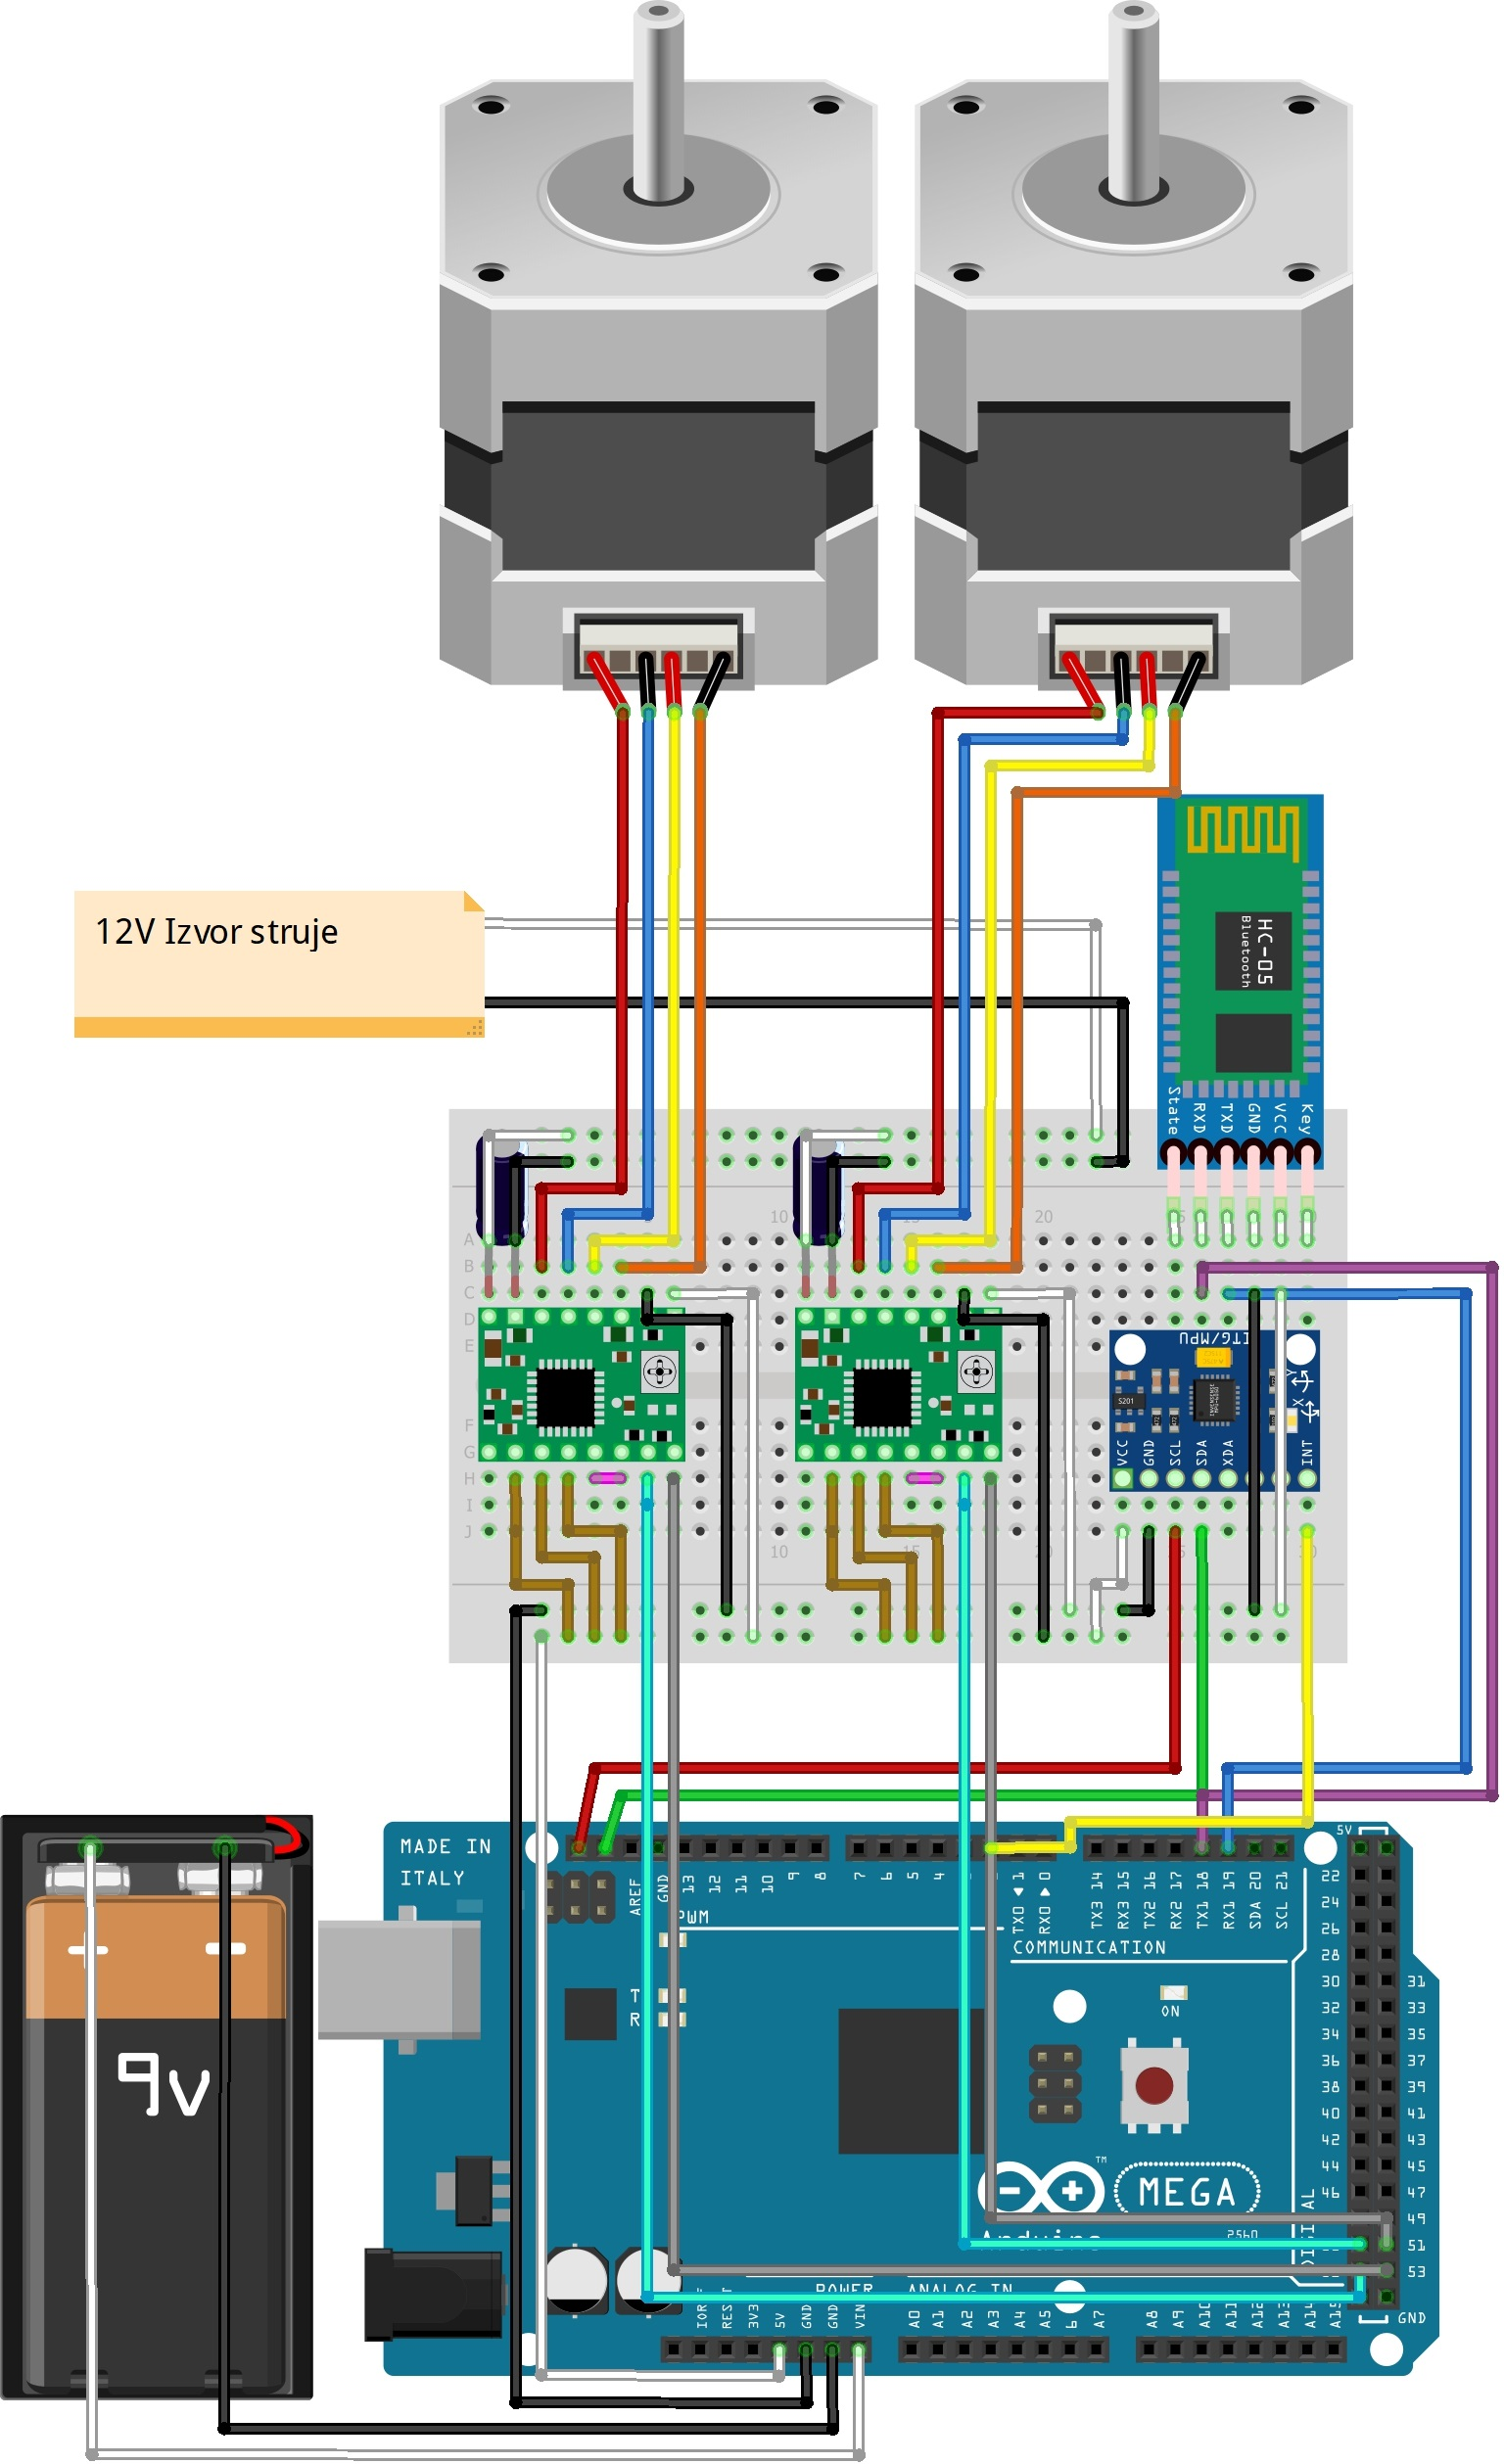
\includegraphics[width=0.8\textwidth]{Robot_Shema}
    \caption{Šema kabliranja robota}
\end{figure}

\subsection{Proces balansiranja}
U procesu balansiranja robota ključna komponenta je MPU6050. Očitavanjem njegovih ulaznih podataka o trenutnom položaju robota u prostoru i prosljeđivanjem tih podataka PID kontroleru (sekcija \ref{pid}), generiše se izlaz koji je proporcionalan brzini motora. Tačnije, kada konstrukcija robota počne padati prema naprijed, PID kontroler će na osnovu podataka iz DMP-a (sekcija \ref{dmp}) poslati signali A4988 upravljaču da kretnjom motora pomjeri robot prema naprijed što će težište motora prilagoditi poziciji njegovog gornjeg dijela te robota zadržati u balansiranom stanju.

\cFigure{Robot_Skica}{Skica sličnog robota}{0.7}

\noindent Pravilo podešene $K_p$, $K_i$ i $K_d$ (sekcija \ref{tuning}), omogućit će da se robot i nakon blagog guranja vrati u balansirano stanje. Promjenom ciljane vrijednosti robot će se kretati naprijed i nazad.

\subsection{Arduino program}
Ključni dio projekta je sami Arduino program koji će kontrolisati robota.

\subsubsection{Biblioteke}
Za izradu programa, korištene su funkcije 5 biblioteka.

\paragraph{PID}\footnote{https://github.com/br3ttb/Arduino-PID-Library}\mbox{}\\
\noindent Ova biblioteka nudi jednostavne funkcije za implementaciju PID kontrolera.
\begin{itemize}
    \item PID(\&y, \&u, \&r, Kp, Ki, Kd) - konstruktor koj prima adrese inicijaliziranih varijabli za ulaz, izlaz i ciljanu vrijednost, kao i parametre za podešavanje
    \item SetOutputLimits(m,n) - postavlja limite izlazne vrijednosti kako bi se izlaz mogao skalirati
    \item SetSampleTime(t) - postavlja vremensku varijablu za kontroler u milisekundama
    \item Compute() - vrši PID kalkulaciju i mijenja vrijednost izlazne varijable
\end{itemize}

\paragraph{TimerOne}\footnote{https://www.arduinolibraries.info/libraries/timer-one}\mbox{}\\
\noindent Pošto će u glavnom programu biti potrebno određene događaje izvršavati na osnovu vremenskog parametra, uključena je biblioteka koja omokogućava podešavanje prekida nakon zadanog vremena.
\begin{itemize}
    \item Initialize(t) - postavlja vrijeme koje će proći između izvršenja prekida
    \item attachInterrupt(void) - zadaje funkciju koja će se izvršiti svakim prekidom.
\end{itemize}

\paragraph{I2Cdevlib}\mbox{}\\
\noindent Ponuđene funkcije ove biblioteke su već opisane u sekciji \ref{itclib}.

\subsubsection{Motors biblioteka}
Prvobitno sam napisao kompletnu biblioteku za akceleraciju i deakceleraciju stepper motora kako bi se robot fluidnije kretao, ali sam kasnije došao do zaključka da će se akceleracija prirodno dogoditi, jer naginjanjem robota PID izlaz postepeno ubrzava motore ka većim brzinama. Ipak mi je jedan dio te biblioteke poslužio i u finalnom projektu.

\begin{itemize}
    \item connectToPins(S,D) - u privatnu varijablu zabilježava pinove ze STEP i DIR na upravljaču motora
    \item setDirection(D) - Postavlja smjer rotacije motora na osnovu enumeratora
    \item makeStep() - Radi 1 korak
\end{itemize}

\begin{code}
    \begin{minted}[breaklines]{cpp}
    void Motor::makeStep()
    {
        digitalWrite(stepPin, HIGH);
        delayMicroseconds(2);
        digitalWrite(stepPin, LOW);
    }

    void Motor::setDirection(Direction Direction)
    {
        if (Direction == Clockwise)
        digitalWrite(directionPin, HIGH);

        if (Direction == CounterClockwise)
        digitalWrite(directionPin, LOW);
    }

    void Motor::connectToPins(byte stepPinNumber, byte directionPinNumber)
    {
        stepPin = stepPinNumber;
        directionPin = directionPinNumber;
        
        pinMode(stepPin, OUTPUT);
        digitalWrite(stepPin, LOW);

        pinMode(directionPin, OUTPUT);
        digitalWrite(directionPin, LOW);
    }
    \end{minted}
    \caption{Funkcije motor klase}
\end{code}

\subsubsection{Tok programa}
Program se može rastaviti na 3 glavna dijela:

\begin{enumerate}
    \item setup()
    \item loop()
    \item prekid
\end{enumerate}

\paragraph{Setup()}\mbox{}\\
\noindent Unutar setup funkcije se inicijaliziraju uređaji.

\begin{enumerate}
    \item Inicijalizacija motora
    \item Otvaranje HC-05 serijske komunikacije
    \item Postavljanje offseta za moju MPU6050 jedinicu
    \item Kalibracija MPU6050
    \item Preuzimanje veličine FIFO paketa od MPU6050
    \item Inicijalizacija vremenskog prekida
\end{enumerate}

\paragraph{Loop()}\mbox{}\\
\noindent Unutar loop funkcije se čeka prekid izazvan od strane MPU6050, te se preuzimaju njegovi paketi i vrši PID kalkulacija

\begin{enumerate}
    \item Ukoliko je broj paketa u FIFO manji od veličine paketa vraća se na početak loop-a
    \item Ukoliko je sa HC-05 došao signal, postavlja se u buffer varijablu
    \item Varijabla koja označava MPU6050 prekid se postavlja na false
    \item Učitavaju se podaci iz FIFO buffera
    \item Podaci iz DMP-a se konvertuju u kvaternion, a zatim u eulerove uglove
    \item Ugao X ose se postavlja kao ulazna vrijednost za PID kontroler
    \item Radi se izračunavanje PID izlaza
    \item Postavlja se smjer motora
    \item Ukoliko je u bufferu neka od komandi za kretanje, aplicira se njen pomak u PID izlaz
    \item Postavlja se vrijeme između koraka za oba motora (brzina motora)
\end{enumerate}

\paragraph{Prekid}\mbox{}\\
\noindent Prekid koji se izvršava na osnovu unutrašnjeg tajmera za zadatak ima pokretanje motora.

\begin{enumerate}
    \item Računanje trenutnog vremena
    \item Računanje vremena od posljednjeg koraka
    \item Poređenje vremena sa PID izlazom
    \item Ukoliko je vrijeme za sljedeći korak
          \begin{enumerate}
              \item Napravi korak
              \item Postavljanje vremena posljednjeg koraka za motor na trenutno vrijeme
          \end{enumerate}
\end{enumerate}

\end{document}